\documentclass[12pt]{article}

\usepackage{float}

\usepackage{standalone}

\usepackage[utf8x]{inputenc}

%%% PAGE DIMENSIONS
\usepackage{geometry}
\geometry{a4paper}
\geometry{margin=2.54cm} % for example, change the margins to 2 inches all round

\usepackage{graphicx} % support the \includegraphics command and options

\usepackage[parfill]{parskip} % Activate to begin paragraphs with an empty line rather than an indent

%%% PACKAGES
\usepackage{booktabs} % for much better looking tables
\usepackage{array} % for better arrays (eg matrices) in maths
\usepackage{paralist} % very flexible & customisable lists (eg. enumerate/itemize, etc.)
\usepackage{verbatim} % adds environment for commenting out blocks of text & for better verbatim
\usepackage{subfig} % make it possible to include more than one captioned figure/table in a single float
% These packages are all incorporated in the memoir class to one degree or another...

\usepackage{multicol}
\usepackage{multirow}
\usepackage{xcolor}
\usepackage{amsmath}

\usepackage[T1]{fontenc}
\usepackage{lmodern}

\usepackage{makecell}

\renewcommand{\arraystretch}{1.1}

%%% HEADERS & FOOTERS
\usepackage{fancyhdr} % This should be set AFTER setting up the page geometry
\pagestyle{fancy} % options: empty , plain , fancy
\fancyhead[L]{\leftmark}
\fancyhead[C]{}
\fancyhead[R]{\rightmark}
\fancyfoot[L]{}
\fancyfoot[C]{}
\fancyfoot[R]{\thepage}
\renewcommand{\headrulewidth}{0pt}
\renewcommand{\footrulewidth}{0pt}

\fancypagestyle{plain}{
	\fancyhf{} % clear all header and footer fields
	\fancyfoot[R]{\thepage} % except the center
	\renewcommand{\headrulewidth}{0pt}
	\renewcommand{\footrulewidth}{0pt}
}

%%% BIBLIOGRAPHY
\usepackage[numbers]{natbib}
\bibliographystyle{vancouver}

%%% SECTION TITLE APPEARANCE
\usepackage{sectsty}
\allsectionsfont{\sffamily\mdseries\upshape} % (See the fntguide.pdf for font help)
% (This matches ConTeXt defaults)

%%% ToC (table of contents) APPEARANCE
\usepackage[nottoc,notlof,notlot]{tocbibind} % Put the bibliography in the ToC
\usepackage[titles,subfigure]{tocloft} % Alter the style of the Table of Contents
\renewcommand{\cftsecfont}{\rmfamily\mdseries\upshape}
\renewcommand{\cftsecpagefont}{\rmfamily\mdseries\upshape} % No bold!

\usepackage[bookmarks,bookmarksnumbered,bookmarksopen,hidelinks]{hyperref}

\usepackage{bookmark}


%%% TITLE
\title{Off-season VE estimates}

\begin{document}

%%% Title
\maketitle

%%% Main Contents

\pagebreak
%
\section{Model}

Assumptions:

\begin{enumerate}
\item All observations are independent.
\item Proportion $p$ of the population is exposed to influenza (is at risk of disease of interest).
\item The unvaccinated have the probability $f$ of infection with influenza.
\item The only differences between the off-season and the during-season populations are $p$ and $f$.
\item Vaccination decreases the probability of infection by influenza by a factor $1 - e$ where $0 \leq e \leq 1$.
\item The entire population is at the same risk $l$ of infection with other respiratory pathogens.
\item Vaccination does not modify the probability of infection with other pathogens.
\item No misclassification (investigated in Section \ref{miss}).
\item The entire infected population (infected by influenza or another pathogen) is included into the test-negative study.
\end{enumerate}

The expected proportions of cases and controls of a test-negative study under the above assumptions in are in Table \ref{ExpectedCounts}.

\begin{table}[htp]
\centering
\caption{
	Expected proportions of a test-negative study under the assumed model. $F$ --- infected with flu (cases). $\bar{F}$ --- infected with a pathogen other than flu (non-cases). $V$ --- vaccinated. $\bar{V}$ --- unvaccinated. $f$ --- probability of flu in unvaccinated. $e$ --- vaccine efficacy. $v$ --- vaccinated proportion. $l$ --- probability of infection by a non-influenza pathogen.
	\label{ExpectedCounts}
}
\begin{tabular}{ccc}
	\toprule
	& $F$ & $\bar{F}$ \\
	$V$ & $pvf(1-e)$ & $vl$ \\
	$\bar{V}$ & $p(1-v)f$ & $(1-v)l$ \\
	\bottomrule
\end{tabular}
\end{table}

The expected odds ratio of a test-negative study is 

\begin{align}
\text{OR}_{\text{TN}}=\frac{pvf(1-e)(1-v)l}{vlp(1-v)f} = 1-e
\label{TNodds}
\end{align}


\pagebreak
%
\section{Low flu activity}

The expected odds ratio of a test-negative study in Eq.\ \ref{TNodds} is unbiased and does not depend on the probability of flu infection $f$. This means that the test-negative VE estimate should be unbiased at any probability of flu infection. Figure \ref{pflu} shows the results of 100,000 simulations of test-negative studies.

\begin{figure}[htp]
	\centering
	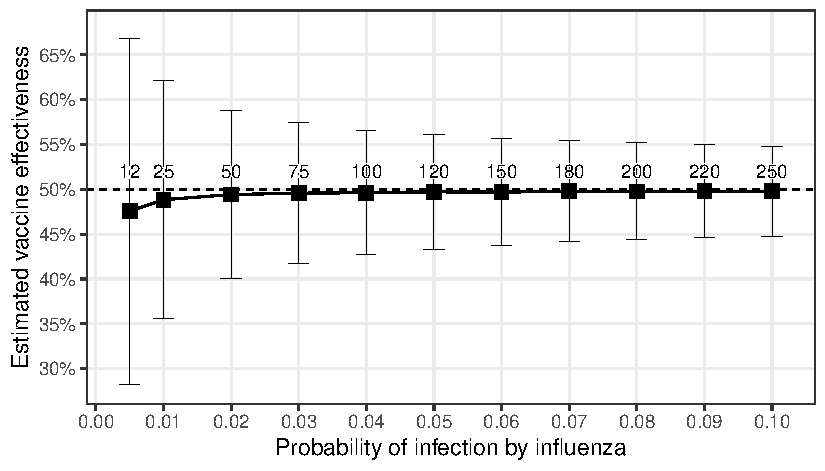
\includegraphics[width=0.8\textwidth]{../graph/pflu.pdf}
	\caption{
	Estimated vaccine efficacy from 100,000 simulations of test-negative studies at different probabilities of flu infection. The true vaccine efficacy was 0.5 (indicated by the dashed line). The points represent probabilities at which the simulations were done. The error bars represent the expected standard deviation of the VE estimate. The numbers represent the expected number of cases in one study. The expected number of controls in all studies was 1,000. The deviation of the mean of the VE estimate across the simulations is negligible due the large number of simulations. The starting population size was 10,000. Everyone in the population was at risk (proportion at risk was 1). The probability of non-influenza infection was 0.1. The vaccinated proportion was 0.5.
	}
	\label{pflu}
\end{figure}

The results in Figure \ref{pflu} show that the estimate remains almost unbiased even at very flu infection probabilities which result in low counts of cases in the test-negative studies. The variation of the estimate across studies predictably decreases with increasing flu infection probability due to the increasing number of cases. 

There is a small (<3\%) amount of bias evident at $f \leq 0.01$. To see where this is coming from, consider Table \ref{GeneralTN} which defines notation for case/noncase counts of a test-negative study. 

\pagebreak

\begin{table}[htp]
\centering
\caption{
	Notation for counts of a test-negative study. $F$ --- infected with flu (cases). $\bar{F}$ --- infected with a pathogen other than flu (non-cases). $V$ --- vaccinated. $\bar{V}$ --- unvaccinated.
	\label{GeneralTN}
}
\begin{tabular}{ccc}
	\toprule
	& $F$ & $\bar{F}$ \\
	$V$ & $X_{c,v}$ & $X_{n,v}$ \\
	$\bar{V}$ & $X_{c,u}$ & $X_{n,u}$ \\
	\bottomrule
\end{tabular}
\end{table}

Under the assumptions of the model, $E(X_{c,v})=vf(1-e)$, $E(X_{c,u})=(1-v)f$, $E(X_{n,v})=vl$, $E(X_{n,u})=(1-v)l$, and so $\frac{E(X_{c,v})E(X_{c,u})}{E(X_{n,v})E(X_{n,u})}$ is unbiased. However, this unbiased quantity is equivalent to the expected VE estimate when the individual counts are averages from many identical studies. The expected VE estimate from one study, $E(\frac{X_{c,v}X_{c,u}}{X_{n,v}X_{n,u}})$ is not the same quantity. The bias that results is related to the fact that the expected value of the reciprocal of a binomial random variable is not the reciprocal of its expected value.

\begin{align}
E(\frac{1}{X}) \neq \frac{1}{E(X)} \quad X \sim \text{Binomial}(n, p)
\end{align}

This bias depends on the expected value, $np$, as shown in Figure \ref{np} more so than it does on the choice of $n$ and $p$ (Figure \ref{npop}).

\begin{figure}[htp]
	\centering
	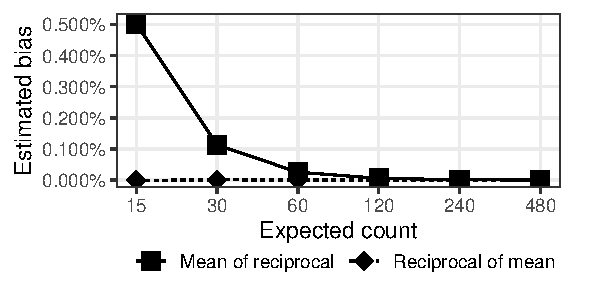
\includegraphics[width=0.7\textwidth]{../binomial-reciprocal/np.pdf}
	\caption{
	Results of simulating random numbers from $\text{Binomial}(n, p)$ where $np$ was set to a value shown on the horizontal axis and $n$ to 500. Points represent values for which 1,000,000 numbers were simulated. The vertical axis shows percent deviation from the true value. Reciprocal of mean means that 1 was divided by the mean taken across all generated numbers (the dashed line). Mean of reciprocal means that 1 was divided by each generated number and the mean taken across the resulting ratios (the solid line).
	}
	\label{np}
\end{figure}

\pagebreak

\begin{figure}[htp]
	\centering
	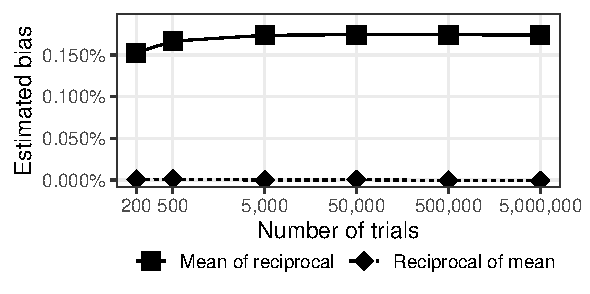
\includegraphics[width=0.7\textwidth]{../binomial-reciprocal/npop.pdf}
	\caption{
	Results of simulating random numbers from $\text{Binomial}(n, p)$ where $n$ was set to a value shown on the horizontal axis and $np$ to 25. Points represent values for which 1,000,000 numbers were simulated. The vertical axis shows percent deviation from the true value. Reciprocal of mean means that 1 was divided by the mean taken across all generated numbers (the dashed line). Mean of reciprocal means that 1 was divided by each generated number and the mean taken across the resulting ratios (the solid line).
	}
	\label{npop}
\end{figure}

The only way to exaggerate this bias any more than it already has been in the simulations in Figure \ref{pflu} would be to decrease the number of controls to very low values as well as cases. I ran an additional set of simulations where both $f$ and $l$ were set to 0.005 (while $p=1$, $v=0.5$, $e=0.5$) with a starting population size of 10,000. The expected number of cases in these simulations was 37.5 and the expected number of controls was 50. The resulting bias was 4.5\% toward the null. So even close to its maximum, this bias is very small and is unlikely to be important in real data.

\pagebreak
%
\section{Inclusion of unexposed population}

If there is a subset of the population that is not exposed to the virus, the people in that subset are at no risk of being infected. Their inclusion into the study may raise concerns but as can be seen from Eq.\ \ref{TNodds}, the odds ratio of a test-negative study does not depend on the proportion of the population ``at risk''. Figure \ref{prisk} summarises simulation results.

\begin{figure}[htp]
	\centering
	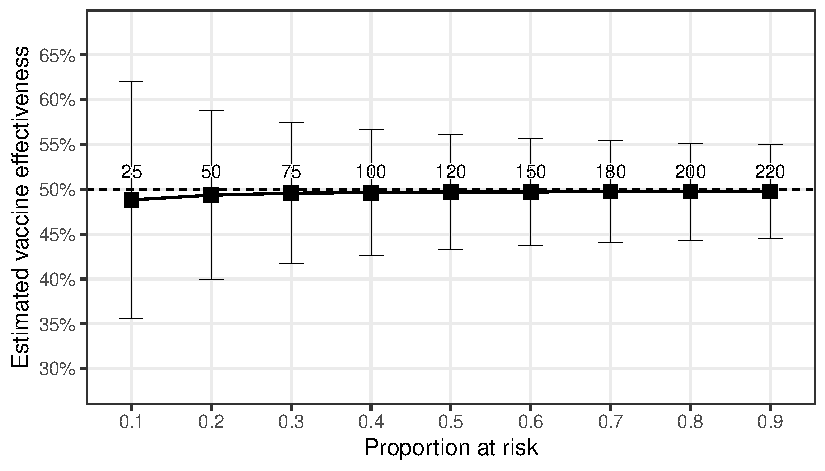
\includegraphics[width=0.8\textwidth]{../graph/prisk.pdf}
	\caption{
	Estimated vaccine efficacy from 100,000 simulations of test-negative studies at different proportions of the sub-population at risk. The true vaccine efficacy was 0.5 (indicated by the dashed line). The points represent probabilities at which the simulations were done. The error bars represent the expected standard deviation of the VE estimate which predictably decreases with proportion at risk due to the increasing number of cases. The numbers represent the expected number of cases in one study. The expected number of controls in all studies was 1,000. The deviation of the mean of the VE estimate across the simulations is negligible due the large number of simulations. The starting population size was 10,000. The probability of flu was 0.1. The probability of non-influenza ARI was 0.1. The vaccinated proportion was 0.5.
	}
	\label{prisk}
\end{figure}

The results in Figure \ref{prisk} mimic those in Figure \ref{pflu}. Under the assumptions, decreasing the proportion at risk is equivalent to decreasing the probability of infection and is not expected to result in notable bias.

In general, the unexposed population will only contribute to the noncase counts. Table \ref{ExpCounts} defines notation for the expected counts of cases and noncases in the total, the exposed and the unexposed populations.

\pagebreak

\begin{table}[htp]
\centering
\caption{
	Notation for counts of a test-negative study in total, exposed and unexposed populations. $F$ --- infected with flu (cases). $\bar{F}$ --- infected with a pathogen other than flu (non-cases). $V$ --- vaccinated. $\bar{V}$ --- unvaccinated.
	\label{ExpCounts}
}
\begin{tabular}{ccc|cc|cc}
	\toprule
	& \multicolumn{2}{c}{Exposed} & \multicolumn{2}{c}{Unexposed} & \multicolumn{2}{c}{Total} \\
	& $F$ & $\bar{F}$ & $F$ & $\bar{F}$ & $F$ & $\bar{F}$ \\
	$V$ & $n_1$ & $n_3$ & $0$ & $n_5$ & $n_1$ & $n_3 + n_5$ \\
	$\bar{V}$ & $n_2$ & $n_4$ & $0$ & $n_6$ & $n_2$ & $n_4 + n_6$ \\
	\bottomrule
\end{tabular}
\end{table}

Under the assumptions, the unbiased odds ratio is $\frac{n_1n_4}{n_2n_3}$. The odds ratio in the general population is $\frac{n_1(n_4+n_6)}{n_2(n_3+n_5)}$.

As long as the vaccinated proportion is the same in the exposed and the unexposed populations, $\frac{n_3}{n_4} = \frac{n5}{n6}=v$ and

\begin{align}
\frac{n_1(n_4+n_6)}{n_2(n_3+n_5)} = \frac{n_1(n_4+n_6)}{n_2(vn_4+vn_6)}=\frac{n_1}{n_2v}=\frac{n_1n_4}{n_2n_3}
\end{align}

Meaning that the expected odds ratio is the same in the total and the exposed populations.

\pagebreak
%
\section{Misclassification} \label{miss}

Misclassification will introduce bias to both the during-season VE estimates and the off-season VE estimates. The off-season estimates may be affected more due to the smaller sample size.

To investigate, I ran the same simulations as reported in Figure \ref{pflu} but in presence of non-differential misclassification described in Table \ref{misstable}. The results are in Figure \ref{pflumiss}.

\begin{table}[htp]
\centering
\caption{
	Parameters of non-differential missclassification used in the simulations.
	\label{misstable}
}
\begin{tabular}{lc}
	\toprule
	Parameter & Value \\
	\midrule
	Sensitivity of vaccination measurement & 0.95 \\
	Specificity of vaccination measurement & 0.8  \\
	Sensitivity of flu test  & 0.86 \\
	Specificity of flu test  & 0.984 \\
	\bottomrule
\end{tabular}
\end{table}

\begin{figure}[htp]
	\centering
	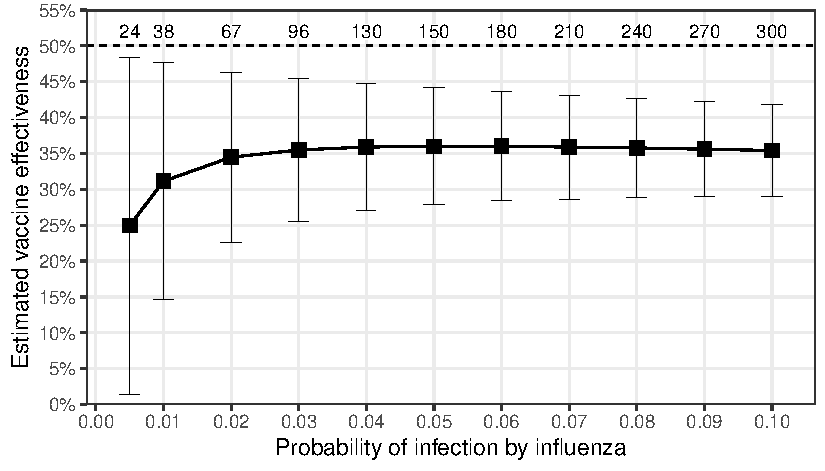
\includegraphics[width=0.8\textwidth]{../graph/pflu-miss.pdf}
	\caption{
	Estimated vaccine efficacy from 100,000 simulations of test-negative studies at different probabilities of flu infection. The true vaccine efficacy was 0.5 (indicated by the dashed line). The points represent probabilities at which the simulations were done. The error bars represent the expected standard deviation of the VE estimate. The numbers represent the expected number of cases in one study. The expected number of controls in all studies was 1,000. The deviation of the mean of the VE estimate across the simulations is negligible due the large number of simulations. The starting population size was 10,000. Everyone in the population was at risk (proportion at risk was 1). The probability of non-influenza infection was 0.1. The vaccinated proportion was 0.5. Parameters associated with misclassification are in Table \ref{misstable}.
	}
	\label{pflumiss}
\end{figure}

\pagebreak

The results show that the VE estimates are more biased in presence of missclassification. This applies to both the during-season (high flu activity) and the off-season (low flu activity) estimates. When flu activity is very low (<0.02), the VE estimates are affected to a greater extent due to the decreased number of cases. 

I ran additional simulations of a very small study (probability of flu and non-flu both set to 0.005). The resulting mean VE estimate was 29\% with a standard deviation of 35\% which is fairly similar to the left-most point in Figure \ref{pflumiss}.

With a smaller number of cases, misclassification has a greater impact on the VE estimates. The smaller number of cases also makes the VE estimates more variable. So while greater bias may be expected from smaller studies (e.g. off-season), the off-season VE estimates cannot be expected to be consistently null (or close to null) under the model assumptions (one of which is that the vaccines still work off-season).

%
\section{Conclusion}

Neither the low flu activity nor the inclusion of the unexposed population can be expected to result in notable bias of VE estimates. If the VE estimates are consistently low when taken off-season, it cannot be explained by the fact that flu activity is low nor by the fact that much of the population is unexposed.

\end{document}
